
\documentclass[11pt,styles/chicago,a4paper]{article}
\usepackage{styles/uereport}
\usepackage{amsthm} % Added by Lucas
\usepackage{url} % added by Lucas
%\usepackage{graphicx} % added by Lucas
\bibliographystyle{abbrv}

\title{Phinishing Phishing: Bridging the Gap \\ Between User and Browser}
\author{Lucas Maystre}
\course{University of California, Berkeley}
\address{lucas@maystre.ch}

\begin{document}
\maketitle

%%%%%%%%%%%%%%%%%%%%%%%%%%%%%%%%%%%%%%%%%%%%%%%%%%%%%%%%%%%%%%%%%%%%%%%%%%%%%%%%

\abstract{
Browsers and users have two different, limited views of a web page. A browser is aware of the request properties, but cannot understand the semantics of the information displayed. A user, on the other hand, understands the information, but does not pay attention to the context. We present a system that brings the user's intention to the browser, reuniting the two views and allowing the browser to take a decisive action. We build a prototypical anti-phishing tool based on our system, and perform a small user study to get an insight on the user's experience. We found out that our approach seems effective in mitigating phishing attacks, and that users find it easy to use even without prior training. % TODO isn't the last sentence a bit too strong?
}

%%%%%%%%%%%%%%%%%%%%%%%%%%%%%%%%%%%%%%%%%%%%%%%%%%%%%%%%%%%%%%%%%%%%%%%%%%%%%%%%

\section{Introduction} %%%%%%%%%%%%%%%%%%

Phishing remains a considerable threat on the web today, causing billions of dollars in damage, according to a 2007 Gartner survey \cite{gartnersurvey}. The difficulty comes from the fact that phishing relies on social engineering techniques exploiting the human nature rather than a technical vulnerability.

On one hand, efficient protection against phishing in the browser space can be reduced to two basic, overlapping problems: the identification of illegitimate web sites, and the actions taken to prevent the leak of information to these sites. If there was a perfect algorithm capable of telling whether a web site is legitimate or not, the second problem would disappear---the request would simply be stopped and an error message would be displayed to the user. However, this is never achieved, resulting in identification errors. Simply dropping the request is therefore not conceivable, as it can block access to a legitimate web site in the case of a false positive, and can have legal consequences \cite{sheng2009improving}. Therefore, mechanisms need to be built in order to alert the user of the potential danger while minimizing the impact of false positives. Solutions, today, range from toolbar security indicators to more active warnings which are harder to overcome.

On the other hand, we can observe that there are two views of a web page: that of the user and that of the browser. The browser sees the request properties, and the raw content. It can even find out additional information such as the location of the server and the registration date of the domain name. But the browser is mostly unable to understand accurately enough the semantics of the information displayed to the user. The user is just in the opposite situation: while he sees the graphical outcome of the request and is able to understand the information displayed, unfortunately he pays little attention to the characteristics of the request such as the domain name or the SSL certificate. At the fundamental level, if either was able to have the understanding of the two views, a correct decision could be made on whether the site is a phishing attack or not. % TODO Acutally, if the DNS is hijacked, it doesn't help. Maybe we can put a footnote for that?

We propose a \emph{resolution system} that combines these two observations and augments existing phishing identification mechanisms by bringing a key piece of information to the browser: the user's intention. When the browser recognizes a web page is suspected of phishing, our system brings the two aforementioned views together and allows the browser to take a decisive action, either allowing or denying the request. This information comes at the cost of interrupting the user but we take great care in designing a system that is simple, usable and resilient to common user mistakes. In practice, our system consists of a user interface mechanism that asks the user: who do you think you are talking to? We motivate the need for a new level of abtraction---the \emph{entity} level---that naturally models the user's intention, and propose a mapping service between entities and domain names. Our system is modular and can be used with any phishing detection system, therefore allowing innovation and improvements. We built a prototypical anti-phishing add-on for Firefox and a simple REST-style API to map entities and domains. Based on this prototype we conducted a small user study, which showed that using our add-on effectively mitigated phishing attacks, and we identified some directions left for future development.

The rest of this paper is organized in the following way: section 2 reviews related work on phishing. Section 3 presents an abstract overview of the solution, while section 4 describes our prototype implementation. In section 5, we present the results of our small user study, and we discuss future work and conclude in section 6.

\section{Related Work} %%%%%%%%%%%%%%%%%

Phishing is a cross-disciplinary problem and involves many stakeholders \cite{sheng2009improving}. % TODO transition is not smooth here...
We focus on the two parts that are the most relevant to our work: the characteristics of phishing, both from the attacker's side and the user's side, and the solutions at the browser level.

\subsection{Characterizing Phishing}

The Anti-Phishing Working Group (APWG) regularly publishes reports on the global state of phishing operations, monitoring various trends among phishers, such as the distribution of domain names and the average uptime of phishing web sites. The global survey over the first half of 2010 \cite{apwg2010h1}, for example, reports a median uptime of 14 hours, and identifies the increasing use of URL shortener services. McGrath \emph{et al.} analyze a large set of phishing URLs together with domain name information and give some insights into phishing operations \cite{mcgrath2008behind}. Among other findings, they point out that phishing domains get active very quickly after registration; they also talk about the hosting infrastructure and argue that botnets play a significant role.

Since phishing web sites use social engineering techniques, which rely on human weaknesses, it is important to look into the human factors of phishing successes. Dhamija \emph{et al.} identify 3 properties that phishing schemes take advantage of: lack of knowledge, visual deception, and bounded attention \cite{dhamija2006why}. Importantly, they point out that security is often a secondary goal. Wu \emph{et al.} review security indicators \cite{wu2006security}, and show that passive security indicators are inefficient, as users often do not look at them.

We leverage these findings to design our solution against a model that takes into account the properties of phishing web sites and human behavior characteristics.

\subsection{Proposed Solutions}

Just like phishing can be characterized by operational and user properties, proposed solutions can also be divided into two categories. The first category contains the technical approaches to identify and block fake web sites. Blacklisting is an important technique, effectively implemented in the major web browsers as of today. Ludl \emph{et al.} quantify its effectiveness \cite{ludl2007effectiveness}. Although important, blacklisting is an incomplete solution, because it does not protect against new phishing attacks.  Many heuristic-based approaches have been developed as well, e.g. based on URL or content properties; we mention CANTINA \cite{zhang2007cantina}, a content-based filter that uses search engine queries to determine whether the displayed page is legitimate. While these approaches are promising, they have often a high false positive rate. We note that these techniques can be incorporated with our solution, as a detection primitive.

On the other hand much effort has been put into solutions in the user interface space. Dynamic security skins \cite{dhamija2005battle} is a mutual authentication mechanism that mitigates risks of spoofing by providing clear visual cues to the user. However, unlike our solution, it requires changes on both the client and the server side. Web Wallet \cite{wu2006web} proposes a virtual wallet used to enter and store sensitive information. To the best of our knowledge, it is the pioneering work that identifies the discrepancy between the browser's and the user's understandings of a web page, and asks for the user's intention as part of the anti-phishing protection. Their solution requires a user to proactively use the wallet before entering sensitive information, whereas we do not require any change of habits. In a sense, our work uses a component of their solution, and makes a full-fledged system from it.

\section{Overview of the Solution} %%%%%%%%%%%%

Broadly speaking, our system is made out of two interacting components: a client-side user interface mechanism implemented in the browser, and a remote database of entities. First, we define and motivate the central concept of \emph{entity}, then we move into a detailed description of the two components.

\newtheorem*{def:entity}{Definition}
\begin{def:entity}
The entity behind a domain name is the organization---company, private individual, etc.---in the name of which the given domain operates legitimately.
\end{def:entity}

The relation between domains and entities is a many-to-many relation: a single entity can of course own several separate domains, and a single domain can operate legitimately in the name of several entities, e.g. a credit card payment processor service. We use entities because we think that they are the closest abstraction of the user's intention when they visit a web site. For example, Internet users want to search on \emph{Google}, not \texttt{google.com}. Another example where the domain name does not necessarily represent the user's intentions is when an operation is delegated---e.g. for a payment processor or in the case of a content delivery network. Furthermore, empirical evidence \cite{facebooklogin} leads us to think that a number of users do not know what a domain name is, and use search engines extensively to get to the web site they intend to visit. Therefore, we adopt entities as the granularity level at which we differentiate the legitimacy of a web site. We think that this approach not only highly correlates with the user's mind when visiting a web site, but also allows any internet user, regardless of knowledge and background to use our system. % Also, motivate the fact that it is the right level of granularity for security!

\subsection{User Interface Plane}

In the browser, we provide a resolution primitive, that can be triggered every time the browser suspects the destination of an HTTP request to potentially steal sensitive information. In practice, this is done by opening a new modal window asking the user's intention. We call it the \emph{resolution window}. We think that a modal window is the right user interface pattern, because the outcome of the resolution defines whether or not the request will be processed further. Ideally, the resolution window should be modal to the browser window or tab from which the request originated, but modeless to the other windows and tab, so as to allow the user to continue to interact with other web sites in parallel.

We ask the user to provide his intention at the entity level, as motivated above. To uniquely identify which entity his intention corresponds to, it has to be selected from a list\footnote{Note that it is possible that the user's intention cannot be matched, e.g. if the site is new and has not yet been added to the database of entites. But at least, we know that the web site is not spoofing any known entity.}. This list can be inferred from web site properties, such as the URL or the text content, but in the generic case, the user queries a list of entities using a search box.

Once the resolution is finished, the browser can match the entity selected by the user with the destination's domain name. If the two match, the resolution is called a \emph{success}, and the browser proceeds further with the request; otherwise, the request is cancelled. On cancellation of a request, the browser displays an informative error page. Because it knows the user's intention, it can personalize the error message and even propose a safe path to the web site the user intended to visit.

\subsection{Entity Database}

To be able to operate at the entity level, there is a need for a new global service mapping entities with domain names, and allowing the user to easily find an entity. For that, we need a comprehensive database of entities. The minimal information needed for the mapping comprises of just two elements: the name of the entity, and a list of domains which are legitimately operating in its name. While these two items are an absolute requirement for our system, we suggest including some other metadata to facilitate the search and to provide a better user experience. We provide a list of information that could be valuable:

\begin{itemize}
\item a graphical representation of the entity, such as a logo
\item name variants, such as short names (e.g. \emph{Chase} instead of \emph{Chase Bank USA, National Association}), and localized names
\item a primary domain name used to redirect the user in the case of a phishing attempt
\end{itemize}

There needs to be a global way to search for entities matching a query string; therefore a natural implementation of the service would be a centralized database, whose access is offered as a service and managed by a trusted third party provider. In a way, this service is comparable to recent DNS resolution services such as Google Public DNS \cite{googledns} or OpenDNS \cite{opendns}.

In fact, only one feature needs to be available centrally: the ability to search through a comprehensive index of entities. All the information associated with an entity---the list of domain names and all other metadata---can be delegated to another service, possibly operated by the entity itself. This can roughly be compared to a DNS resolution, where the central index plays the role of a root server. For every entity found in the centralized index, a second request is sent to the resolution service authoritative for the the entity. This decoupling allows entities to retain more control over the metadata. Arguably, it also allows the resolution system to scale better: the minimal amount of data stored in the central index is likely to change at a slower rate than the complete set of data associated with the entity, and this load can be distributed across many auxiliary mapping services.

\begin{figure}[t]
  \genfig{figures/distributedlookup}{5.5}
  \caption{The distributed lookup mechanism. The browser first queries a list of entities from the central index, and then obtains the associated metadata through the auxiliary service authoritative for the entity.}
  \label{fig:distriblkp}
\end{figure}

Figure \ref{fig:distriblkp} shows a diagram for this two-step resolution process. The browser first sends a query to the central index. The central index returns, for each entity matching the query, a unique entity identifier and the location of the authoritative mapping service. The browser then sends a second request to the mapping service, which finally replies with the information associated with the entity. The authentication of the auxiliary mapping services could be implemented using a public key scheme, where the central index plays the role of a certification authority.

\section{Prototype Implementation} %%%%%%%%%%%

We implemented an anti-phishing add-on prototype as a simple instance of the system proposed in the previous section. The focus of this prototype was on the user interface, because we were interested in testing the user experience.

\subsection{Resolution Triggering}

In the previous section, we showed how the resolution mechanism works. In practice, it would be unacceptable to trigger a resolution for every page visited. To lower the burden on the user, the goal is to trigger the resolution only when there is a \emph{risk} associated to the request. A variety of existing or proposed phishing detection mechanisms can be used for that purpose. In the case of our prototype, we use a simple whitelist based mechanism. We first observe that, as long as the user does not input data into the web page, there is no information leak. Therefore, we trigger our decision process only when the user inserted data in the web page---we detect this by listening to keyboard events.

To decide whether the domain is suspect, we use a widespread community-managed web site trust indicator, Web of Trust \cite{wot}. WOT provides a public API \cite{wotapi}. Domain reputation is rated across four components, each having a confidence rating. We only look at the trustworthiness component and impose a threshold on both its value and its confidence. If a domain does not attain the threshold in one or the other, or is not found in the WOT database, it is considered suspect. This effectively achieves a whitelist approach: the only requests that do not require resolution are those that are known and reasonably trusted. A thorough discussion about whether this particular phishing detection is effective in detecting malicous web sites is outside the scope of this paper, but we informally checked our decision algorithm against a feed of live phishing sites \cite{phishtank}, and it yielded positive results.

As already mentioned, the triggering component is conceptually separate from the rest of the system. Therefore, any heuristic can be used and advances in detection techniques will directly translate into improvements for our system.

\begin{figure}[t]
  \genfig{figures/decisiondiagram}{3.5}
  \caption{The resolution triggering decision process. A resolution is triggered only when there's a possible data leak, and when the request destination is suspect.}
  \label{fig:decisiondgrm}
\end{figure}

\subsection{Entity API}

We have designed a simple mapping service, which we call the \emph{Entity API}. It provides REST-style HTTP API with just one functionality: get a list of entities and their metadata, given a search query string. Technically, this was implemented using a PostgreSQL relational database storing the entities and their associated information, and a simple PHP script interfacing the request to the database and formatting the output into an XML document. For every entity matching the query the data sent back to the client contains:

\begin{itemize}
\item a long name (e.g. \emph{Chase Bank USA, National Association})
\item a short name (e.g. \emph{Chase})
\item a list of domains, including a primary domain to which the user can be redirected, in case the resolution fails
\item the network location of a representative image of standard dimensions (128$\times$128 pixels)
\end{itemize}

The search query is matched against the long name, the short name, and the domain names. We use several techniques to increase our search engine's resilience to spelling mistakes; for example we compute the soundex key \cite{knuth1973art} to search for names that sound similarly. The client queries the service through a simple URL (e.g. \texttt{http://chi.lum.li/entities/Pay\%20pall}), and receives an XML document back.

\subsection{Firefox Add-on}

On the browser side, we decided to implement the user interface mechanism as an add-on for Firefox \cite{Firefox}. We chose Firefox because it has a significant market share---around 25\% in November 2010 \cite{statcounter, netapplications}, and it allows rapid and easy prototyping of add-ons. Other security extensions have been proposed for Firefox in the past \cite{samuel2009requestpolicy}. Figure \ref{fig:screenshots} shows what the resolution window looks like when prompting the user to enter a query and when displaying the list of entities. We also included an error page (not shown in the figure) displayed when a mismatch between the selected entity and the domain name is detected. This page contains a link to safely reach the entity and a search box pre-filled with the entity's name.

\begin{figure}[t]
  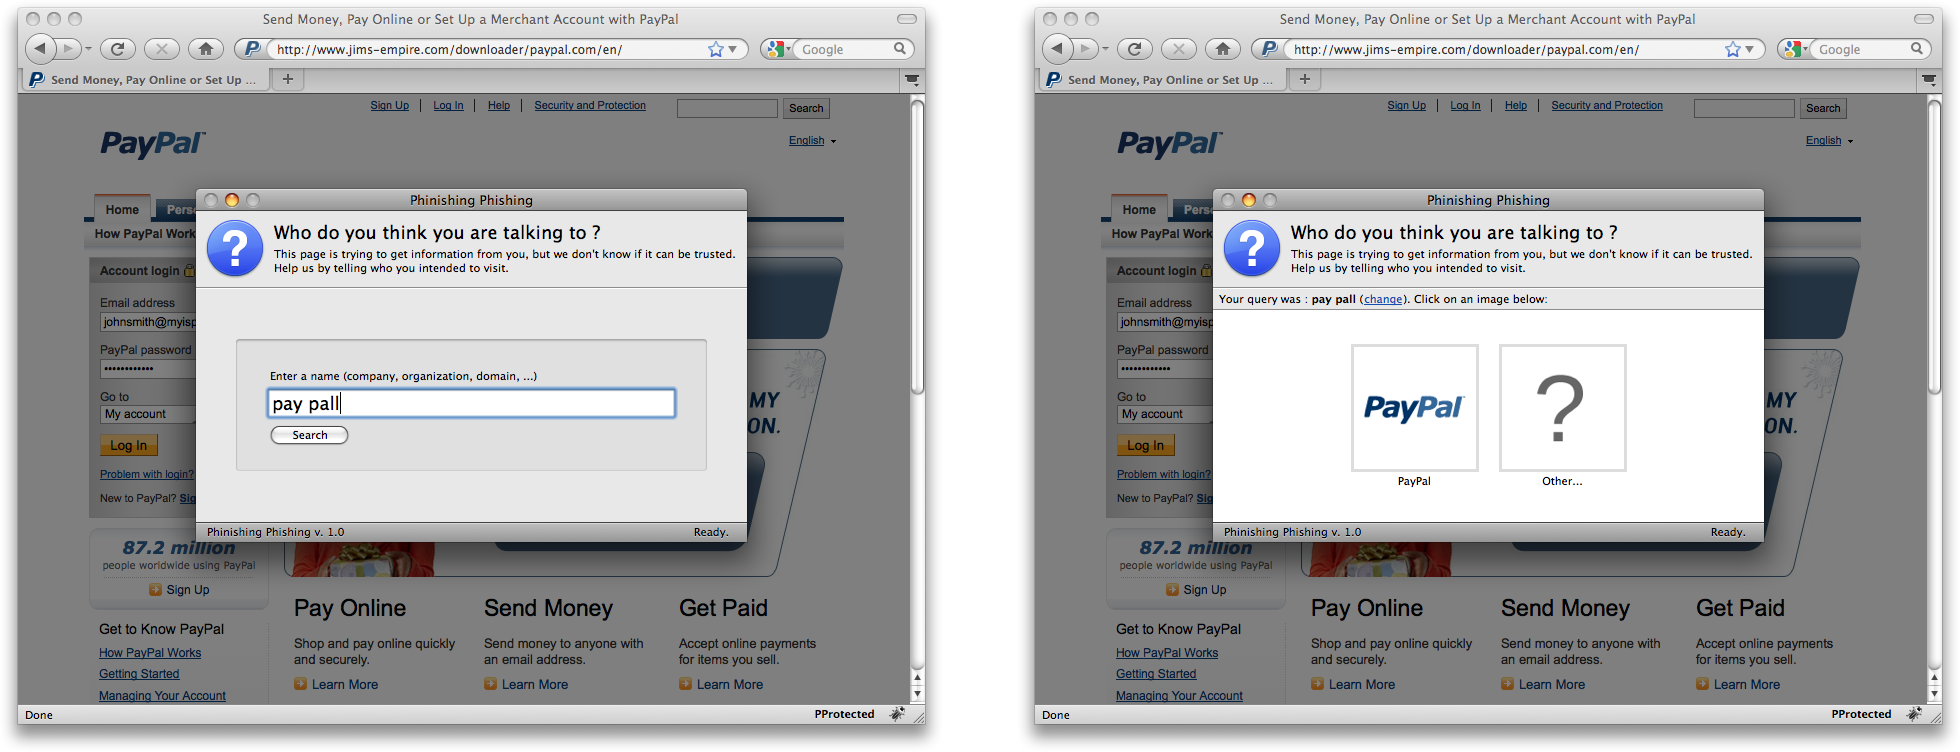
\includegraphics[width=\textwidth]{figures/screenshots.png}
  \caption{The resolution window. The user can search in the Entity Database, and picks from a list of matching entities. The lookup is resilient to spelling mistakes.}
  \label{fig:screenshots}
\end{figure}

\section{User Study} %%%%%%%%%%%

We conducted a small user study to get some insights into the system from a user's perspective. We recruited 20 subjects, one of whom did not complete the study. Out of these 19 subjects, 17 were undergraduate or graduate students with a wide range of majors; one subject was a high school student, and one was a school teacher. Their age ranged from 15 to 52. % TODO correct the ages
They were all using Firefox as their main browser before the study, and were instructed to use only Firefox for the entire duration of the study. Afterwards, we administered an anonymous survey to get, among other things, an idea of what kind of technical background they had, for which we received 15 responses. 20\% of the responding subjects declared not knowing what a domain name is. 53\% had never or barely heard of phishing, while 73\% had never or barely heard of SSL certificates.

We do not claim that our subjects are representative of any class of population, in any way. We conducted the study for two reasons: to get an understanding of how users experience our prototype and interact with it, and to see if it can help preventing data leakage on phishing web sites.

The study followed roughly the same scenario as in \cite{wu2006web}: the subjects were told to play the role of Jane, the assistant to John Smith. They were given a list of Smith's account credentials on 6 popular web sites (eBay, PayPal, Amazon.com, LinkedIn, Twitter, Craigslist). Once or twice a day, they would receive an e-mail asking them to perform a small task, involving logging into one of the sites. For example, one of the tasks could have been to log into eBay and to get the price of an auction item previously added to the watchlist. The study lasted 5 days, over which 7 tasks were sent. These e-mails contained a link taking the subject to the site on which they could accomplish the task. Out of the 7 e-mail that were sent, two of them contained a link to an illegitimate web site under our control. If they were logging into the illegitimate web sites, we would log the access and redirect them to the legitimate web site. The subjects were not told that the experience was about phishing or anything related to security. The only information given about the extension was that \emph{sometimes a window could pop up and ask them something}.

\subsection{Results}

We divided the subjects randomly into two groups: one which had the extension installed (9 subjects), and one which didn't (10 subjects). The spoof rate---defined as the number of compromised accounts divided by the number of e-mails sent---was 11\% for the first group and 100\% for the second group. The result for the second group was surprising, and we first thought that they might have misunderstood the task. At the end of the study, we posed some questions to the subjects of the second group. They did not notice anything special, except for a few of them who remembered having needed to enter their login information twice. We justify this extreme result by the authority of the e-mail sender. The subjects trusted him, and did probably not think much when following his instructions. The impact of social structures on phishing has been studied by Jagatic \emph{et al.} \cite{jagatic2007social}.

The result of the first group is very positive, showing that in the vast majority of the cases, we successfully protected the user from falling for the illegitimate web sites. However, out of the 18 malicious e-mails sent out to this group, 2 of them still succeeded---it is natural to wonder what was in cause. After the study finished, we contacted the two subjects, which both told us that the resolution window did not appear for that task. We also investigated our logs, and indeed it seems that due to an undetermined bug in the add-on the resolution window did not open properly, and our mechanism got bypassed.

\begin{figure}[t]
  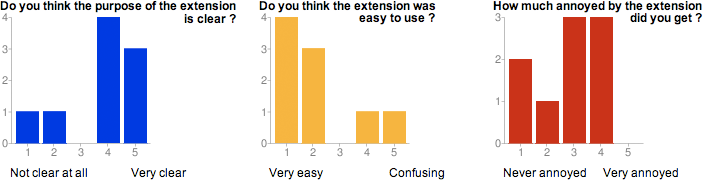
\includegraphics[width=\textwidth]{figures/experience.png}
  \caption{Histograms of answers to user experience related questions. All the 9 subjects that used the extension replied to the survey.}
  \label{fig:experiences}
\end{figure}

In the survey we administered after the study we included several questions specifically for the add-on group, about their experience. Figure \ref{fig:experiences} shows the answers we got for three of the questions. As we can see, the add-on was rather intuitive and easy to use---remember that we gave no training or explanations to the subjects. On the other hand, we can say that the annoyance caused by the extension was significant. By discussing with the subjects and looking at our logs, we discovered two main sources of annoyances:

\begin{enumerate}
\item The resolution was sometimes triggered for well known web sites, such as Amazon.com or Google. The reason is that these web sites often use content delivery networks to serve static objects and the domain names of these objects' URL are not rated in the WOT trust database.
\item When navigating a suspect domain, the add-on keeps triggering a resolution every time a request is done and the user inputs data. This turned out to be problematic e.g. for AJAX intensive webmails that were not in the whitelist. There was no way for the user to permanently add a domain to the whitelist.
\end{enumerate}

We are confident that these technical difficulties are not fundamental flaws of our system, but are tied to the specifics of the prototype and can be overcome.


\section{Future Work \& Conclusion} %%%%%%%%%%%

While this preliminary study has shown the potential for the solution, there are still several aspects that need to be studied more thoroughly to have a complete system. In this section, we review some of the issues left for future work.

\begin{description}
\item[Entity Management] The management of the Entity Database is arguably one of the more complex parts of the system. A set of protocols and mechanisms needs to be provided to allow entities to manage their entry in the index. The whole resolution infrastructure needs to be more clearly defined.

\item[Privacy] When a resolution is triggered, the user has to divulge his intention to the entity index. While the loss of privacy doesn't appear to be excessive (in our opinion it is comparable to the use of a search engine), especially given the low rate at which we hope to trigger the resolution, we think that this issue deserves to be studied in detail.

\item[Input Sources] If the resolution mechanism is triggered only when user input has been detected on the web page, all the sources have to be characterized and watched to guarantee security. Our prototype only listens to key strokes on HTML text input boxes (\texttt{<input>} and \texttt{<textarea>} tags), but these are not the only input possibilities. External plug-ins (Java applets, Flash animations) also provide input mechanisms. We are aware that some web sites use virtual keyboards where the user clicks on images of characters to thwart keyloggers; this technique can also be exploited by attackers. Other less common input sources include audio---via a microphone---and video---via a webcam.

\item[Whitelisting] The study identified that users can get annoyed when they have to resolve the same site more than once. But whitelisting all domains for which we triggered the resolution once opens the way to a new kind of attack, where the attacker first displays a harmless page, and, after the first visit and the resolution displays a malicious phishing page. The resolution, instead of being associated with the domain name, should be associated with a \emph{semantic snapshot} of the page, so that if the displayed information changes completely, the resolution is triggered again. More work is needed to find out how this can be done, but this problem tends to solve itself naturally when using a content-based detection heuristic.

\item[User Experience] We are aware that the additional burden we require might slow down user adoption. Specifically, we speculate that having to type the name of the entity is a burden that is an order of magnitude worse than just clicking on the entity's image. Therefore, we should focus on developing techniques to better infer the intention, and offer a one-click resolution experience in most of the cases.

\item[Changes to the Threat Model] While our prototype seemed to offer an effective protection against typical phishing attacks we observe today, we have not considered how an attacker could try to overcome or even \emph{take advantage} of our system. There is a need to investigate new threats, for example at the entity management level. 

\end{description}

As mentioned in the introduction, phishing is a problem spanning many domains and we do not claim that this is a complete solution that eradicates the threat. Nevertheless, we think that our system is a step forward in providing strong defense at the browser level.

\section*{Acknowledgments}
We would like to thank Scott Shenker, who suggested the idea of asking the user which web site he wants to visit and proposed the title of this paper. Thank you also to Ion Stoica, for the insightful comments at the beginning of the project. A big thank you to Trung Le Dang for his help with the user study, Tony Lin for his careful review, and Ana\"elle Maillard.

\bibliography{references}


\end{document}

